\documentclass{article}
\usepackage{amsmath, amssymb, amsthm, enumerate, framed, graphicx}
\usepackage[usenames,dvipsnames]{color}
\usepackage{hw}
\usepackage{bm}
\usepackage[colorlinks=true,urlcolor=blue]{hyperref}
\usepackage{geometry}
\geometry{margin=1in}
\usepackage{float}
\setlength{\marginparwidth}{2.15cm}
\usepackage{booktabs}
\usepackage{enumitem}
\usepackage{epsfig}
\usepackage{setspace}
\usepackage{tikz}
\usepackage{parskip}
\usepackage[]{algorithm2e}

\newcommand{\comment}[1]{\textcolor{blue}{\textsc{\textbf{[#1]}}}}

% Some commands to allow solutions to be embedded in the assignment file.
\ifcsname issoln\endcsname \else \def\issoln{1} \fi
\newcommand{\soln}[1]
{
  \if\issoln 1
  \textbf{Solution:}
  #1
  \fi
}
\newcommand{\norm}[1]{\lVert #1 \rVert}
\newcommand{\st}{\mathrm{s.t.}}

\makeatletter
\newcommand{\removelatexerror}{\let\@latex@error\@gobble}
\makeatother

\begin{document}

\section*{}
\begin{center}
  \centerline{\textsc{\LARGE Homework 3}}
  \vspace{1em}
  \centerline{\textsc{\Large Support Vector Machines and Neural Networks}}
  \vspace{1em}
  \textsc{\large CMU 10-701: Machine Learning (Fall 2018)} \\
  \textsc{Authors: Yang Gao, Sarah Mallepalle, Umang Bhatt}
  \centerline{OUT: Oct 3}
  \centerline{DUE: Oct 17, 11:59 PM}
\end{center}


\section*{START HERE: Instructions}


\begin{itemize*}
\item \textbf{Collaboration policy:} Collaboration on solving the homework is allowed, after you have thought about the problems on your own.  It is also OK to get clarification (but not solutions) from books or online resources, again after you have thought about the problems on your own.  There are two requirements: first, cite your collaborators fully and completely (e.g., ``Jane explained to me what is asked in Question 3.4'').  Second, write your solution {\em independently}: close the book and all of your notes, and send collaborators out of the room, so that the solution comes from you only.

\vspace{0.1in}
\item\textbf{Submitting your work:} Assignments should be submitted as PDFs using \href{https://gradescope.com/}{Gradescope} unless explicitly stated otherwise.  Submissions written in latex are preferred however handwritten submissions are also allowed, please follow the instructions below for each format:\\
\textbf{Latex:} If you are submitting a Latex document each derivation/proof written between the begin\{soln\} and the end\{soln\} for that specific question. \\
\textbf{Handwritten:} Submissions can be handwritten in which case please submit each solution on a seperate page. You are in charge of making sure your solutions are legible if we cannot read your solutions you will not be given credit for them.\\
Upon submission, label each question using the template provided by Gradescope. 

\vspace{0.1in}
\item \textbf{Programming}: All programming portions of the assignments should be submitted to \href{https://autolab.andrew.cmu.edu/courses/10701-f18/assessments}{Autolab}.  We will not be using this for autograding, meaning you may use any language which you like to submit.
\end{itemize*}

\newpage

\section*{Problem 1: Support Vector Machine [20 pts]}
In this question, we are considering the kernel version of SVMs:
$$ \min_{\omega \in \mathbb{R}^d, b, \xi_i \in \mathbb{R}, i=1,2,...,n} \frac{1}{2} ||\omega||^2_2 + C \sum_{i=1}^n \xi_i $$
 $$ s.t. \quad y^{(i)}(\omega^T \phi(x)^{(i)}+b) \geq  1- \xi_i, \forall i=1,...,n $$
$$\xi_i \geq 0, \forall i=1,...,n$$
where $x^{(i)} \in \mathbb{R}^p, i=1,2,...,n$ is the original training data coming along with the label $y^{(i)} \in \left\{-1,1\right\}, C>0$, is a constant and $\phi: \mathbb{R}^p \leftarrow \mathbb{R}^d$ is a mapping function that maps the original data to a new space. Generally speaking, $d>p$ (In fact, $d$ can be $+\infty$). Please answer the following questions. Note that the questions with complexity could be answered with big-O notation.
\subsection*{1.1 Lagrangian form and dual problem [8 pts]}
Given the above functions, the Lagrangian form of SVM is
$$ L(\omega,b, \xi, \alpha, \eta)=\frac{1}{2}||\omega||^2_2 + C \sum_{i=1}^n \xi_i- \sum_{i=1}^n \alpha_i[y^{(i)}(\omega^T\phi(x^{(i)})+b)+\xi_i-1]- \sum_{i=1}^n\eta_i \xi_i $$
where $\alpha, \eta \in \mathbb{R}^n$ are the dual variables.
Now the max-min form of the dual problem is
$$\max_{\alpha \geq 0, \eta \geq 0} \min_{\omega, b, \xi} L(\omega, b, \xi, \alpha, \eta)$$
Please derive the simplified expression of the dual problem, in terms of just $\alpha$, step by step. \\

\begin{soln}
        % Type solution here
\end{soln}

\pagebreak 

\subsection*{1.2 Primal solution and Kernel SVM [12 pts]}
Suppose we have obtained the solution of the dual problem, denoted as $\alpha_i^\star$ for $i = 1,2,...,n$. Following the course slides, we know that the primal solution is
$ \omega^\star = \sum_{i=1}^n \alpha_i y^{(i)} \phi (x^{(i)})$, $b^\star = y^{(k)}-\sum_{i=1}^n \alpha_i y^{(i)} \langle \phi(x^{(i)}), \phi(x^{(k)}) \rangle$,  for any $k$ that $0 < \alpha_k < C$. Write down the corresponding primal solution $\omega^\star$ and $b^\star$. In the sub-questions below, suppose we now have to use the kernel SVM to make a classification decision at some test data point $z \in \mathbb{R}^p$. (12 points, 4 for each subproblem)
\begin{enumerate}
\item {What is the time complexity of making the classification decision if the mapping is given by
{\small $$ \phi(x) = ( \underbrace{p^2, x_{p-1}^2, \cdots, x_1^2}_{\text{p}}, \underbrace{\sqrt[]{2}x_p x_{p-1},\cdots, \sqrt[]{2}x_p x_1}_{\text{p-1}}, \underbrace{\sqrt[]{2}x_{p-1} x_{p-2}, \cdots , \sqrt[]{2}x_{p-1} x_1}_{\text{p-2}}, \cdots, \sqrt[]{2}x_2 x_1, \sqrt[]{2c}x_p,\cdots,\sqrt[]{2c}x_1,c)^T,$$}
with a constant $c > 0$, and we need to compute it from scratch?
}

\begin{soln}
    % Type solution here
\end{soln}

\hfill \linebreak

\item Let $K(u,v) = \phi(u)^T \phi(v)$ where $\phi(\cdot)$ has the same definition as above. Please give a compact form of $K(u,v)$. What is the time complexity of making the classification decision if we directly compute $K(\cdot, \cdot)$?

\begin{soln}
    % Type solution here
\end{soln}

\hfill \linebreak

\item Now please go back to the dual formulation you derived previously. To avoid repetitive computation, one can precompute all the inner products $K(x^{(i)}, x^{(j)}) = \phi(x^{(i)})^T \phi(x^{(j)})$ before solving the dual problem. What is the space complexity of this approach and what might be a problem if $n$ is huge?

\begin{soln}
    % Type solution here
\end{soln}

\end{enumerate}


\newpage
\section*{Problem 2: Perceptron [20 pts]}
\subsection*{2.1 Proving convergence in linear separability [10 pts]}

Consider the scenario where we are using linear classifiers (passing through origin) as our learning model ($h(\mathbf{x}) = sign (\mathbf{w^T x}))$, and the perceptron algorithm as our learning algorithm. Given a dataset of n samples of d-dimensional vectors ($\mathbf{x_i}$) with class labels ($y_i$), where the labels can take only 2 values $+1$ or $-1$, assume that there exists a weight vector $\mathbf{w^*}$ that linearly separates the positive and negative samples, such that:

\begin{equation}
y_i (\mathbf{w^*})^T \mathbf{x_i} \geq \gamma, \forall i
\label{eq1}
\end{equation}

where, $\gamma > 0 (\gamma \in \mathbb{R})$, 
$\mathbf{x_i} \in \mathbb{R}^d$, 
$y_i \in \{+1, -1\}$, 
$\mathbf{w^*} \in \mathbb{R}^d$. 

The perceptron algorithm starts with $\mathbf{w^{(0)}} = \mathbf{0}$ (superscript denotes update-step number), and updates the weight vector at the $k$th step when it encounters a misclassified sample, $\mathbf{w^{(k)}} = \mathbf{w^{(k-1)}} + y_k \mathbf{x_k}$. A sample $(\mathbf{x},y)$ is misclassified (at a step $i$) if:
\begin{equation}
 y {\mathbf{(w^{(i-1)})}^T \mathbf{x}} \leq 0 
 \label{eq2}
\end{equation}

Assume further that for all training input vectors, the $L_2$ norm is bounded, $||\mathbf{x_i}||_2 \leq V$ ($\forall i = 1 .. n$).

Show that the number of updates ($t$) to the weight vector starting from $\mathbf{w^{(0)}} = 0$ in such a scenario is bounded by $\frac{V^2 ||\mathbf{w^*}||^2_2}{\gamma^2}$.

For proving this result:
\begin{enumerate}
    \item Try to lower bound $\mathbf{w^*}^T\mathbf{w^{(t)}}$, using Equation \ref{eq1}. Specifically show that $\mathbf{w^*}^T\mathbf{w^{(t)}} \geq t\gamma $.
    \item Now, upper bound $||\mathbf{w^{(t)}}||^2$ using the update rule (Equation \ref{eq2}), and show that $||\mathbf{w^{(t)}}||^2_2 \leq t V^2 $.
    \item Now use the above two parts to get the desired result. (Hint: use cosine of $\mathbf{w^*}$, $\mathbf{w^{(t)}}$)
\end{enumerate}

\begin{soln}
        % Type solution here
\end{soln}

\newpage

\subsection*{2.2 Implementing perceptron algorithm [10 pts]}
Let's consider the linear classification model with a bias term, 
\begin{equation}
h(\mathbf{x}) = sign (\mathbf{w^T x} + b)
\label{df}
\end{equation}
where $sign(v)$ outputs $+1$ if $v \geq 0$, and $-1$ otherwise. 

The perceptron learning algorithm can be expressed as follows (for a given dataset $D = \{\mathbf{x_i}, y_i\}, i = 1..n , \mathbf{x_i} \in \mathbb{R}^d, y_i \in \{+1, -1\}$):



This algorithm can be used to obtain $\mathbf{w}$ and $b$, which can then be used to predict labels of the test samples using equation \ref{df}. Implement this algorithm for the task of classification on the data given in Piazza Resources as \texttt{HW3\_Q2\_Data.zip}. Report your accuracy on the test set, and the number of iterations it took  the algorithm to converge on the training set.

\begin{algorithm}
\SetKwInOut{Input}{input}\SetKwInOut{Output}{output}

Let  $\mathbf{w = 0}$, $i = 0$, $numIter = 100$  \\
\While{!(all samples correctly classfied) AND $i < numIter$}
{
\For{$s = 1, 2, .. n $}  
  {
  \If{ $y_s(\mathbf{w^T x_s} + b) \leq 0$}{
    $\mathbf{w} = \mathbf{w} + y_s \mathbf{x_s}$\;
    $b = b + y_s$ \;
   }

	}
	$i = i + 1$ \;
	}
\Return $\mathbf{w}, b, i$
\caption{Perceptron algorithm on training samples}
\label{alg:pa1}
\end{algorithm}

\begin{soln}
        % Type solution here
\end{soln}


\newpage
\section*{Problem 3: Neural Networks [25 pts]}

Consider the following two layer neural network architecture in the figure below.
\begin{figure}[!htbp]
\begin{center}
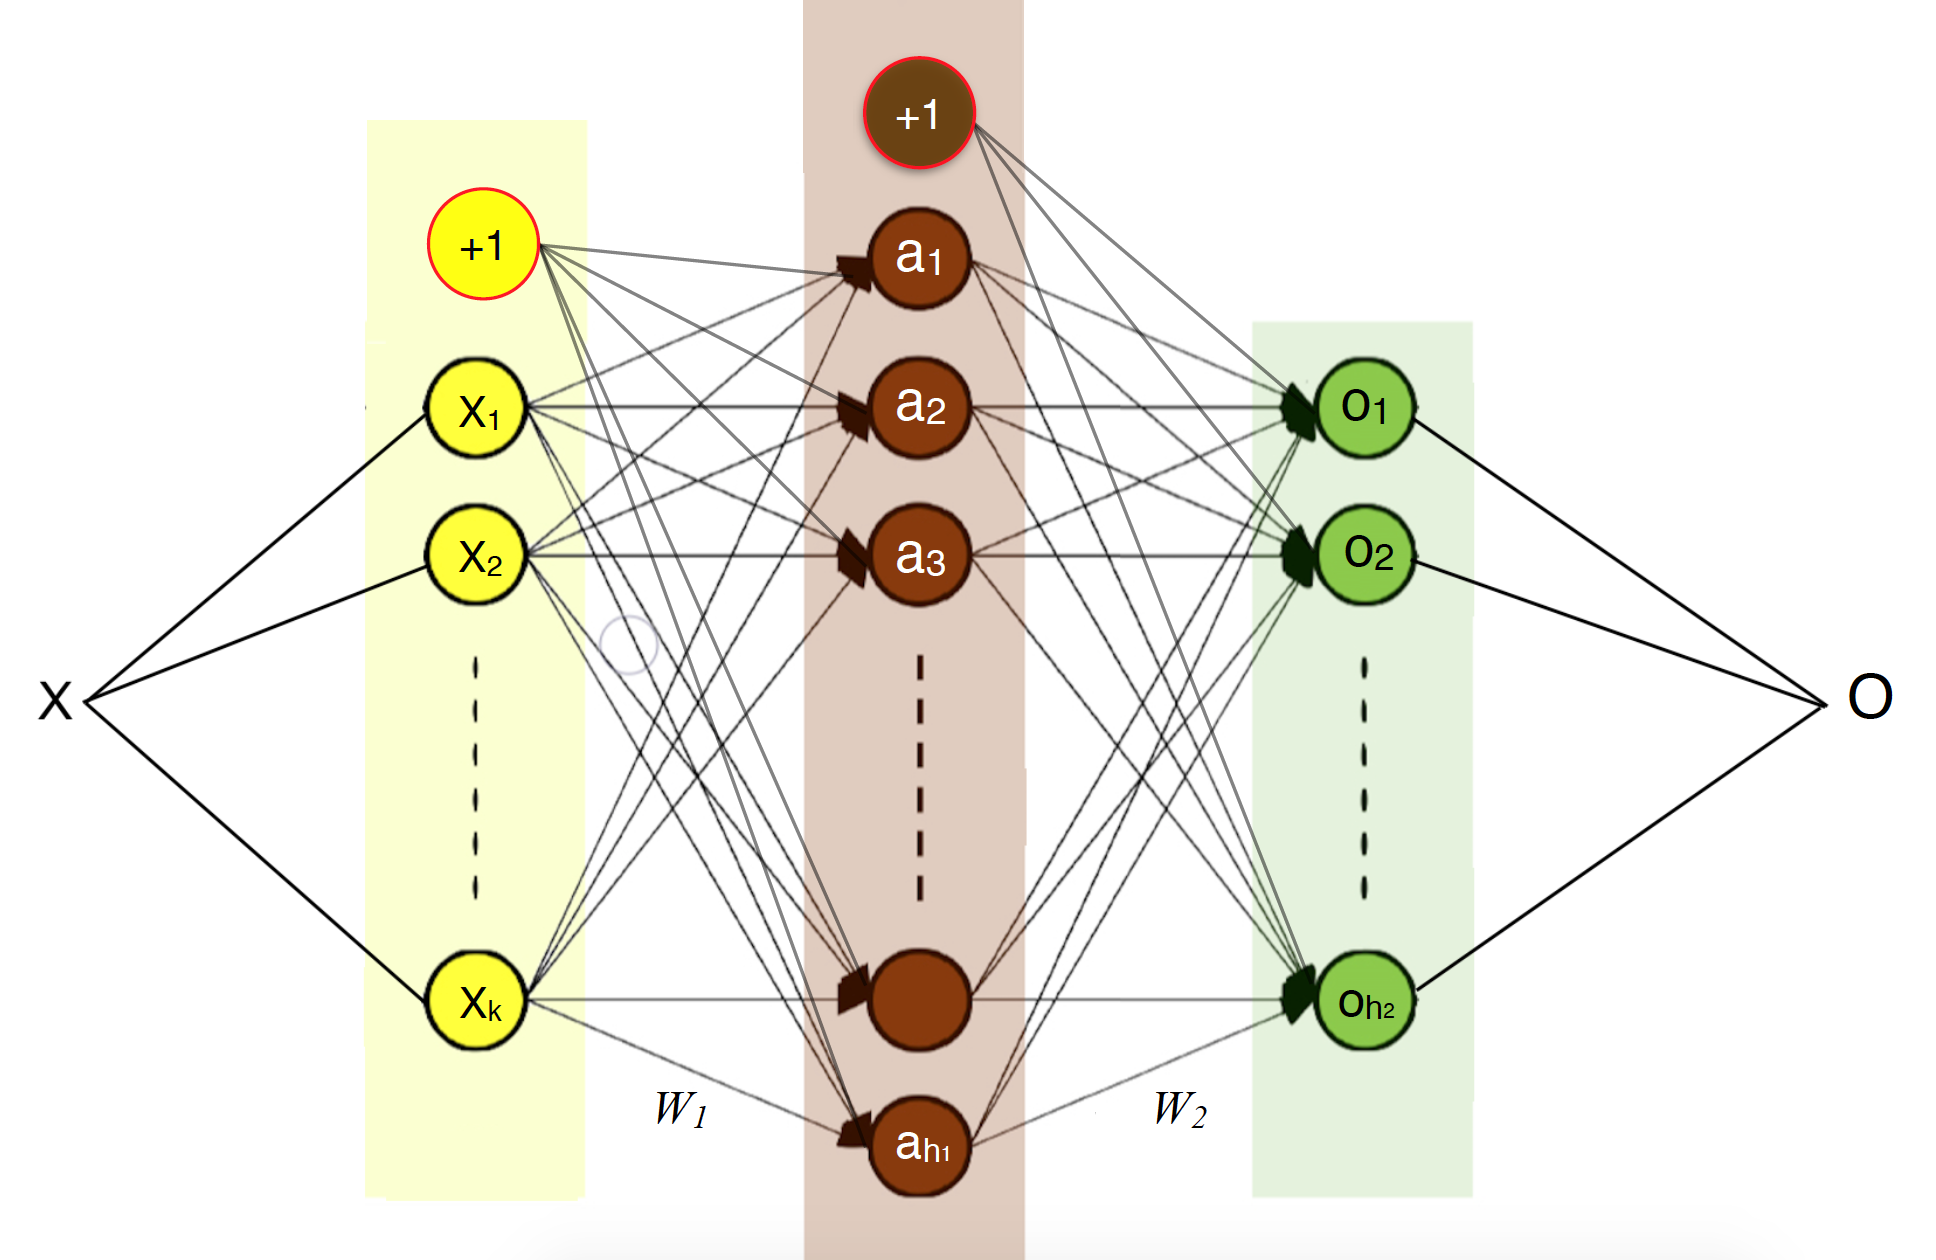
\includegraphics[width = 0.9\textwidth]{plots/revised_nn.png}
\end{center}
\end{figure}

The output of the network can be written as a function of the neural network parameters:
\begin{align*}
	f = \underbrace{S(\underbrace{\underbrace{g(\underbrace{xW_1 + b_1}_{f_1})}_{a}W_2 + b_2}_{f_2})}_{o}
\end{align*}

The specifications of the network are as follows:
\begin{itemize}
\item $x$ is a single data point of shape $1 \times k$. 
\item $g$ is an activation function - either the \textbf{sigmoid} or the \textbf{tanh} function for the purposes of this problem.
\item $S$ is the softmax function.
\item $h_{1}$ is the number of hidden units in layer 1 and $h_{2}$ is the number of hidden units in layer 2. 
\item $f$ is the output matrix of shape $1 \times h_{2}$.
\item $a$, $o$ are the activations of the hidden and output layer, of shapes $1 \times h_1$ and $1 \times h_2$, respectively.
\item $W_{1}$, $W_{2}$ are weight matrices of shape $k \times h_{1}$ and $h_{1} \times h_{2}$,  respectively.
\item $b_{1}$, $b_{2}$ are bias vectors of shape $1 \times h_{1}$ and $1 \times h_{2}$, respectively.
\end{itemize}

\pagebreak

So, we have that:
\begin{tabbing}
\hspace*{2cm}\=\hspace*{3cm}\= \kill
 \hspace*{10mm} $f_1 =$ \> $xW_1+b_1$ \> shape $1 \times h_1$, the linear combination output $f_1$ of $x$ using $W_1$\\
 \hspace*{10mm} $a =$ \> $g(f_1)$ \> shape $1 \times h_1$, the nonlinear activation function output $a$\\
 \hspace*{10mm} $f_2 =$ \> $aW_2+b_2$ \> shape $1 \times h_2$, the linear combination output $f_2$ of $a$ using $W_2$\\
 \hspace*{10mm} $o =$ \> $S(f_2)$ \> shape $1 \times h_2$, the softmax output $o$ of $f_2$\\
\end{tabbing}

In this problem, we will consider neural networks constructed using the following two types of non-linear activation functions: 
\begin{itemize}
\item \textbf{sigmoid} $\sigma(x)$ = $\frac{1}{1 + e ^{-x}}$
\item \textbf{tanh} tanh(x) = $\frac{e^{2x}-1}{e^{2x}+1}$
\item \textbf{softmax} $S_i(x)$ = $\frac{e^{x_i}}{\sum_j{e^{x_j}}}$
\end{itemize}

\hfill \linebreak
Furthermore, we will use the Cross Entropy Loss given by:
\begin{equation*}
	Error(network) = -\sum_{i = 1}^{ {h_2}} y_i\log y'_i,
\end{equation*}
where $y_i$ $\in\{0,1\}$ is the target label, and $y'_i$ is the $i^{\text{th}}$ predicted output of the network.
\newline\newline

\subsection*{3.1 Reveal the Black box [20 pts]}
Derive the backpropagation algorithm with respect to the adjustable parameters of this network, using (a) \textbf{sigmoid $\sigma(x)$} as the activation function and (b) \textbf{tanh} as the activation function. Note: consider softmax activation for layer 2 in both cases (a) and (b). 

\begin{soln}
    % Type solution here
\end{soln}

\subsection*{3.2 Neural Networks Meet Logistic Regression [5 pts]}
Recall that Logistic Regression models the conditional probability of a label $Y\in\{0,1\}$ given $p$-dimensional input $X\in\mathbb{R}^{p}$ as:
\begin{equation*} \label{eq:prob1}
P(Y=0|X=x)=\frac{1}{1 + \exp(w^T x)}
\end{equation*}
and
\begin{align*}
P(Y=1|X=x) &= 1- P(Y=0|X=x)\\
&= \frac{\exp(w^T x)}{1 + \exp(w^T x)},
\end{align*}
where $w\in \mathbb{R}^{p}$ denotes a weight vector.\newline\newline
Using only sigmoid and linear activation functions, create a Neural Network that for a three-dimensional input $X\in\mathbb{R}^{3}$  behaves like an ensemble of two Logistic Regression classifiers. Note that a Linear Activation function has the form $L(x) = C \, (w^T \, x)$, where $x$ is an input vector, $w$ is a weight vector, and $C$ is a constant; and by ensemble of classifiers here we simply mean a weighted linear combination of classifiers.

\begin{soln}
    % Type solution here
\end{soln}




\newpage
\section*{Problem 4: Multiple Choice [5 pts]} 

\def\layersep{2.5cm}

\begin{enumerate}[noitemsep]
    \begin{figure}[H]
    \centering
    \begin{tikzpicture}[shorten >=1pt,->,draw=black!50, node distance=\layersep]
        \tikzstyle{neuron}=[circle,fill=black!25,minimum size=17pt,inner sep=0pt]
        \tikzstyle{input neuron}=[neuron, fill=green!50];
        \tikzstyle{output neuron}=[neuron, fill=red!50];
        \tikzstyle{annot} = [text width=4em, text centered]
        \foreach \name / \y in {1,...,5}
            \node[input neuron] (I-\name) at (0,-\y) {};
        \node[output neuron, right of=I-3] (O) {};
        \foreach \source in {1,...,5}
            \path (I-\source) edge (O);
        \node[annot,above of=I-1, node distance=1cm] (il) {Input layer};
        \node[annot,right of=il] {Output layer};
    \end{tikzpicture}
    \end{figure}
    \item \textbf{[1 pt]} What is the most common name of the neural network shown in the figure above, when sigmoid activation functions are being used?
    \begin{enumerate}
        \item Perceptron
        \item Kernel Regression
        \item Logistic Regression
        \item Capsule Network
    \end{enumerate}

    \begin{soln}
        % Type solution here
    \end{soln}

    
    \hfill \linebreak
    
    \item \textbf{[1 pts]} What does the decision boundary of the neural network shown in the figure above look like when sigmoid activation functions are being used?
    \begin{enumerate}
        \item Logistic
        \item Quadratic
        \item Linear
        \item Non-linear
    \end{enumerate}

    \begin{soln}
        % Type solution here
    \end{soln}

     \pagebreak
     
    \begin{figure}[H]
    \centering
    \begin{tikzpicture}[shorten >=1pt,->,draw=black!50, node distance=\layersep]
        \tikzstyle{neuron}=[circle,fill=black!25,minimum size=17pt,inner sep=0pt]
        \tikzstyle{input neuron}=[neuron, fill=green!50];
        \tikzstyle{output neuron}=[neuron, fill=red!50];
        \tikzstyle{hidden neuron}=[neuron, fill=blue!50];
        \tikzstyle{annot} = [text width=4em, text centered]
        \foreach \name / \y in {1,...,4}
            \node[input neuron] (I-\name) at (0,-\y) {};
        \foreach \name / \y in {1,...,7}
            \path[yshift=1.5cm]
                node[hidden neuron] (H-\name) at (\layersep,-\y cm) {};
        \node[output neuron, right of=H-4] (O) {};
        \foreach \source in {1,...,4}
            \foreach \dest in {1,...,7}
                \path (I-\source) edge (H-\dest);
        \foreach \source in {1,...,7}
            \path (H-\source) edge (O);
        \node[annot,above of=H-1, node distance=1cm] (hl) {Hidden layer};
        \node[annot,left of=hl] {Input layer};
        \node[annot,right of=hl] {Output layer};
    \end{tikzpicture}
    \end{figure}
    
    \item \textbf{[2 pts]} Now consider the model shown in the figure above, instead of the previous one. Why might this be a better model?
    \begin{enumerate}
        \item It has a faster training and inference time than that of a linear model.
        \item It requires less space in memory to store model parameters when compared to logistic regression.
        \item It learns a non-linear decision boundary.
        \item It will underfit to the data, making it easy to train with less data.
    \end{enumerate}

    \begin{soln}
        % Type solution here
    \end{soln}
    
    \hfill \linebreak
    \item \textbf{[1 pts]} We use hinge loss a surrogate loss for 0/1 loss, because hinge loss is:
    \begin{enumerate}
        \item Convex and differentiable
        \item Differentiable but not convex
        \item Convex but not differentiable 
        \item Neither convex nor differentiable 
    \end{enumerate}

    \begin{soln}
        % Type solution here
    \end{soln}
    
\end{enumerate}




\newpage
\section*{5 Programming Exercise (20 pts)}
\subsection*{5.1 Tensor Flow Playground for Neural Networks [5 pts]}
In this problem we will use the TensorFlow playground \href{http://playground.tensorflow.org}{http://playground.tensorflow.org}, which is a nice visual tool for training simple Multi Layer Perceptrons (MLPs).
Your goal in this problem is to carefully select input features to design the ``smallest'' MLP classifiers that can achieve low test loss for each of the 4 datasets in TensorFlow playground (Figures 1 - 4 show the 4 datasets available on TensorFlow playground). Note that you have to design a separate classifier for each individual dataset.  Here \emph{smallest} is defined as having least number of neurons in the network. By low test loss we mean a test loss $< 0.1$ for the swiss roll dataset and a test loss of $\approx 0$ for the rest of the datasets. Submit screenshots after your networks achieve the required test loss for each of the datasets.

\begin{figure}[!htb]
\minipage{0.23\textwidth}
  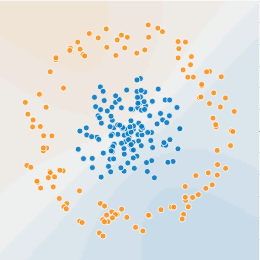
\includegraphics[width=\linewidth]{plots/Circles}
  \caption{Circles}\label{}
\endminipage\hfill
\minipage{0.23\textwidth}
  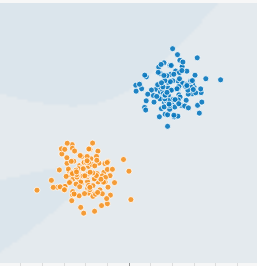
\includegraphics[width=\linewidth]{plots/Clusters}
  \caption{Clusters}\label{}
\endminipage\hfill
\minipage{0.23\textwidth}
  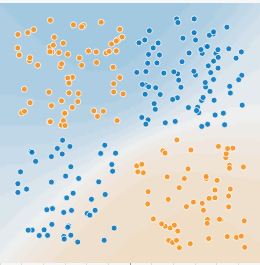
\includegraphics[width=\linewidth]{plots/Squares}
  \caption{Squares}\label{}
\endminipage\hfill
\minipage{0.23\textwidth}
  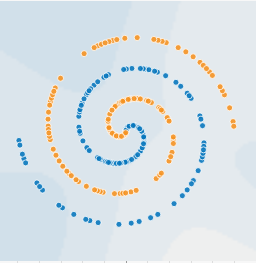
\includegraphics[width=\linewidth]{plots/SwissRoll}
  \caption{Swiss Roll}\label{}
\endminipage
\end{figure}

\begin{soln}
        % Type solution here
\end{soln}



\subsection*{5.2 Binary Classification [15pts]}
In this problem you will be using a binary (two class) version of \emph{mnist} dataset. The data and code template can be downloaded from Piazza Resources as \texttt{HW3\_Q5\_Data.zip}.

We use the following formulation in this problem:
\[
\min_{w\in \mathbb{R}^d}   \frac{\lambda}{2} \|w\|^2_2 + \frac{1}{n}\sum_{i = 1}^n \max(1 - y_i\left\langle w, X_i\right\rangle, 0).
\]
This is only done to simplify calculations. You will optimize this objective using Stochastic Sub-Gradient Descent (SSGD) (Shalev et. al., 2011). This approach is very simple and scales well to large datasets\footnote{To estimate optimal $w$, one can also optimize the dual formulation of this problem. Some of the popular SVM solvers such as LIBSVM solve the dual problem. Other fast approaches for solving dual formulation on large datasets use dual coordinate descent.}. In SSGD we randomly sample a training data point in each iteration and update the weight vector by taking a small step along the direction of negative ``sub-gradient'' of the loss\footnote{Sub-gradient generalizes the notion of gradient to non-differentiable  functions}. \pagebreak

The SSGD algorithm is given by:
\begin{itemize}
\item Initialize the weight vector $w = 0$.
\item For t = 1 \dots T 
\begin{itemize}
\item[*] Choose $i_t \in \{1, \dots n\}$ uniformly at random
\item[*] Set $\eta_t = \frac{1}{\lambda t}$.
\item[*] If $y_{i_t}\left\langle w, X_{i_t}\right\rangle < 1$ then:
\begin{itemize}
\item[--] Set $w \leftarrow (1- \lambda\eta_t)w + \eta_ty_{i_t}X_{i_t}$
\end{itemize}
\item[*] Else:
\begin{itemize}
\item[--] Set $w \leftarrow (1- \lambda\eta_t)w$
\end{itemize}
\end{itemize}
\item Return $w$
\end{itemize}
Note that we don't consider the bias/intercept term in this problem. 

\begin{itemize}
\item Complete the \texttt{train(w0, Xtrain, ytrain, T, lambda)} function in the \texttt{svm.py} file (\textttt{matlab} users complete the \textfff{train.m} file).
\begin{itemize}

\item The function \texttt{train(w0, Xtrain, ytrain, T, lambda)} runs the SSGD algorithm, taking in an initial weight vector \texttt{w0}, matrix of covariates \texttt{Xtrain}, a vector of labels \texttt{ytrain}. \texttt{T} is the number of iterations of SSGD and \texttt{lambda} is the hyper-parameter in the objective. It outputs the learned weight vector \texttt{w}.
\end{itemize}
\item Run \texttt{svm\_run.py} to perform training and see the performance on training and test sets.
\end{itemize}

\paragraph{Evaluation}
\begin{itemize}
\item Use \texttt{validation}  dataset for picking a good \texttt{lambda($\lambda$)} from the set \texttt{\{1e3, 1e2, 1e1, 1, 0.1\}}.
\item Report the accuracy numbers on train and test datasets obtained using the best \texttt{lambda}, after running SSGD for $200$ epochs (i.e., $T = 200*n$).  Generate the training accuracy vs. training time and test accuracy vs training time plots.
\end{itemize}

\begin{soln}
        % Type solution here
\end{soln}



\end{document}